\documentclass[11pt,letterpaper]{article}

\addtolength{\oddsidemargin}{-.875in}
\addtolength{\evensidemargin}{-.875in}
\addtolength{\textwidth}{1.75in}

\addtolength{\topmargin}{-.875in}
\addtolength{\textheight}{1.75in}

\usepackage[utf8]{inputenc}
\usepackage{caption} % for table captions
\usepackage{amsmath} % for multi-line equations and piecewises
\DeclareMathOperator{\sign}{sign}
\usepackage{graphicx}
\usepackage{relsize}
\usepackage{xspace}
\usepackage{verbatim} % for block comments
\usepackage{subcaption} % for subfigures
\usepackage{enumitem} % for a) b) c) lists
\newcommand{\Cyclus}{\textsc{Cyclus}\xspace}%
\newcommand{\Cycamore}{\textsc{Cycamore}\xspace}%
\newcommand{\deploy}{\texttt{d3ploy}\xspace}%
\newcommand{\Deploy}{\texttt{D3ploy}\xspace}%
\usepackage{tabularx}
\usepackage{color}
\usepackage{multirow}
\usepackage{float} 
\usepackage[acronym,toc]{glossaries}
%\include{acros}
\definecolor{bg}{rgb}{0.95,0.95,0.95}
\newcolumntype{b}{X}
\newcolumntype{f}{>{\hsize=.15\hsize}X}
\newcolumntype{s}{>{\hsize=.5\hsize}X}
\newcolumntype{m}{>{\hsize=.75\hsize}X}
\newcolumntype{r}{>{\hsize=1.1\hsize}X}
\usepackage{titling}
\usepackage[hang,flushmargin]{footmisc}
\renewcommand*\footnoterule{}
\usepackage{tikz}

\usetikzlibrary{shapes.geometric,arrows}
\tikzstyle{process} = [rectangle, rounded corners, 
minimum width=1cm, minimum height=1cm,text centered, draw=black, 
fill=blue!30]
\tikzstyle{arrow} = [thick,->,>=stealth]

\graphicspath{}

\begin{document}

\section{3D-neutronics}

\subsection{3D-unitcell}

	\begin{itemize}
		\item Input file: \textit{3D-unitcell.i}
		\item Mesh: \textit{3D-unitcell.msh}
		\item Transient problem.
	\end{itemize}

Figure \ref{fig:3D-unitcell} displays the geometry.
Figure \ref{fig:3D-unitcell1} shows the results.

	\begin{figure}[htbp!]
		\centering
		\begin{subfigure}[t]{0.4\textwidth}
			\centering
			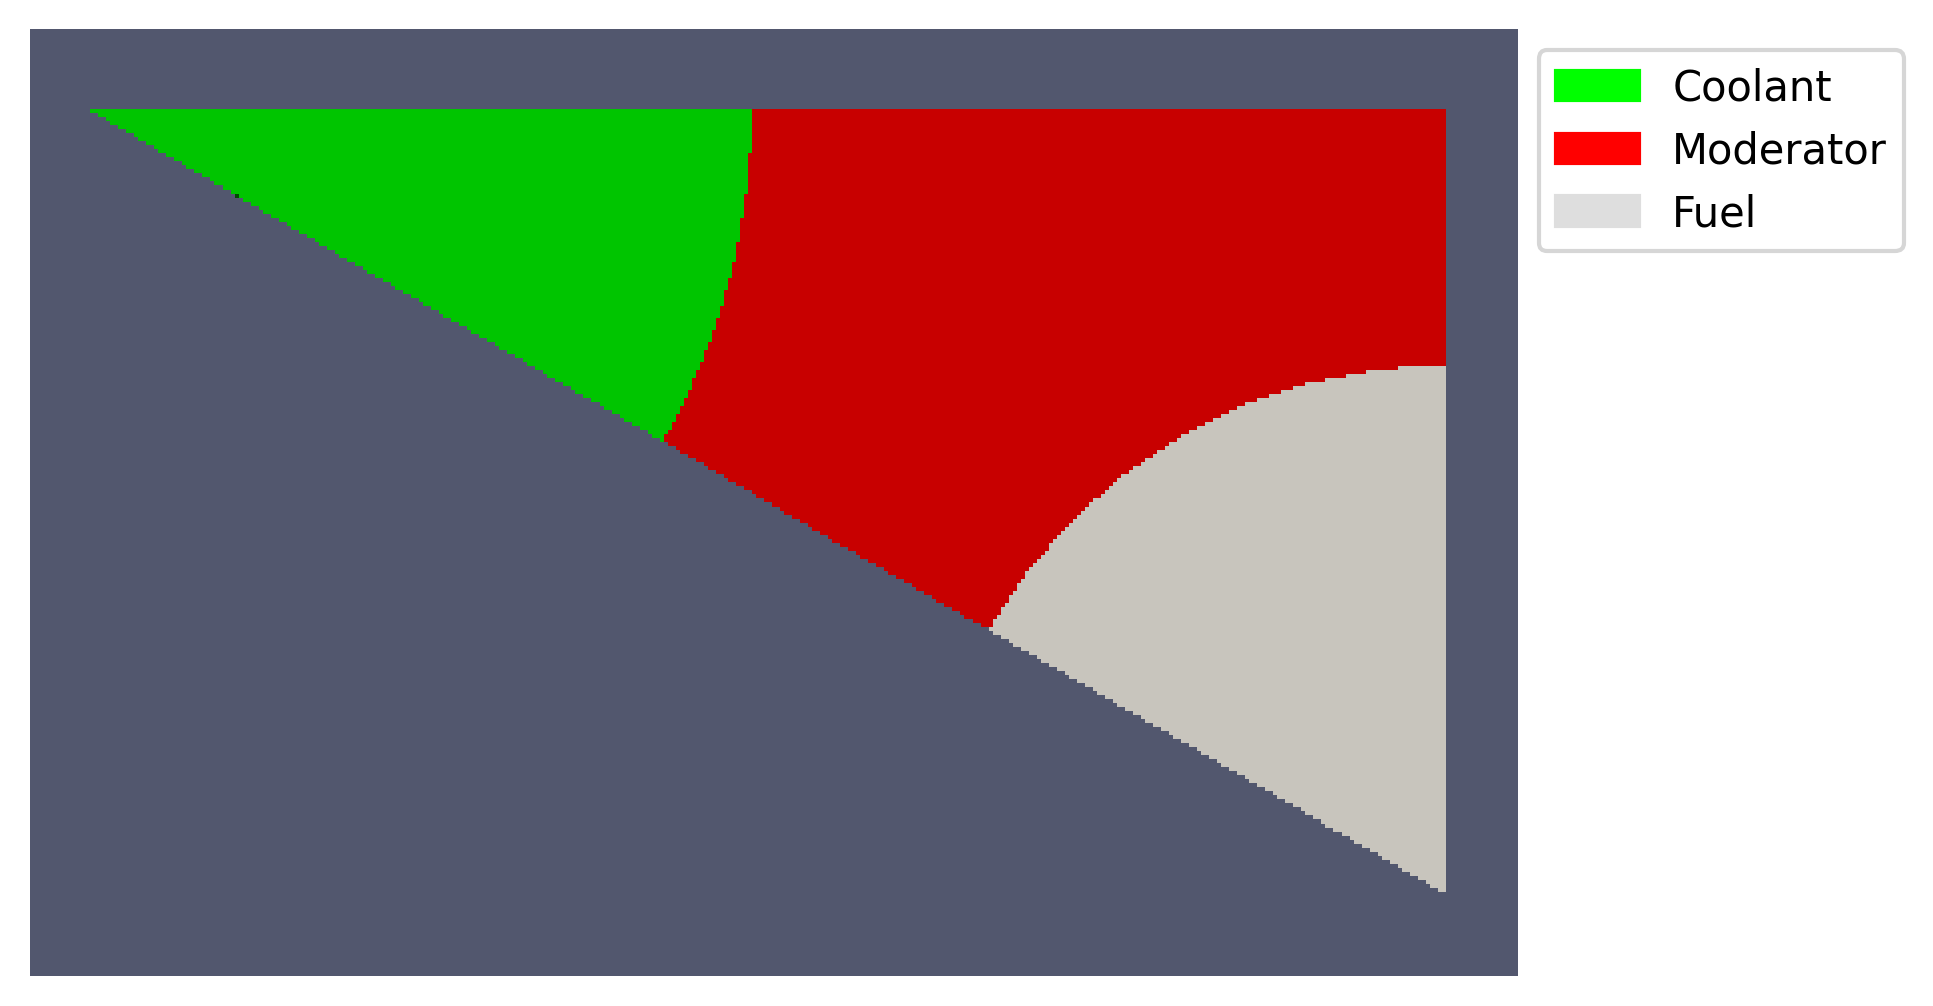
\includegraphics[width=\linewidth]{3D-unitcell-mesh1}
			\caption{XY-plane.}
		\end{subfigure}
		\begin{subfigure}[t]{0.4\textwidth}
			\centering
			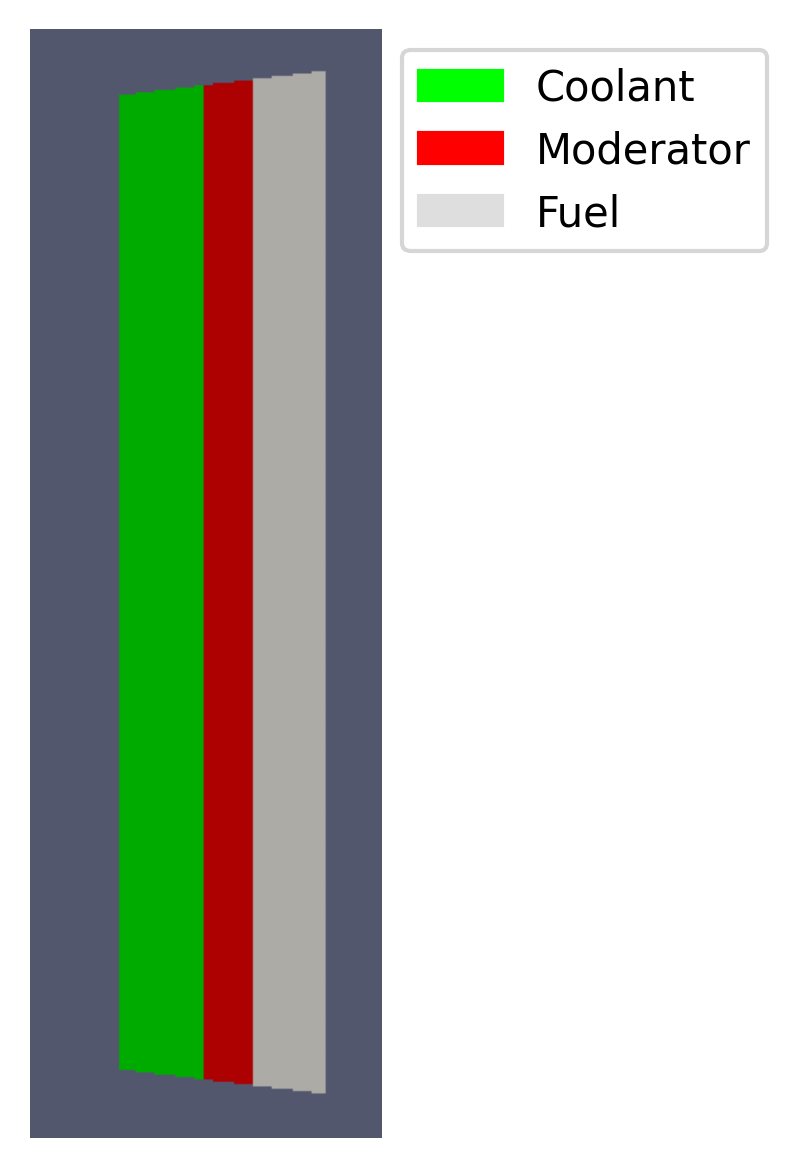
\includegraphics[width=\linewidth]{3D-unitcell-mesh2}
			\caption{XZ-plane.}
		\end{subfigure}
		\hfill
		\caption{\textit{3D-unitcell} scaled down geometry.}
		\label{fig:3D-unitcell}
	\end{figure}

	\begin{figure}[htbp!]
		\centering
		\begin{subfigure}[t]{0.4\textwidth}
			\centering
			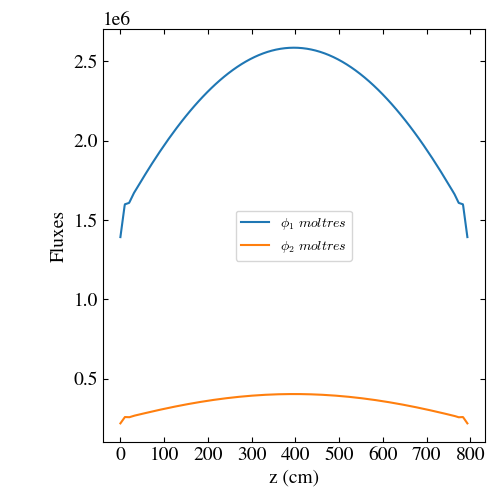
\includegraphics[width=\linewidth]{3D-unitcell1}
			\caption{Fuel centerline between points (1.628,-0.939,0) and (1.628,-0.939,793).}
		\end{subfigure}
		\begin{subfigure}[t]{0.4\textwidth}
			\centering
			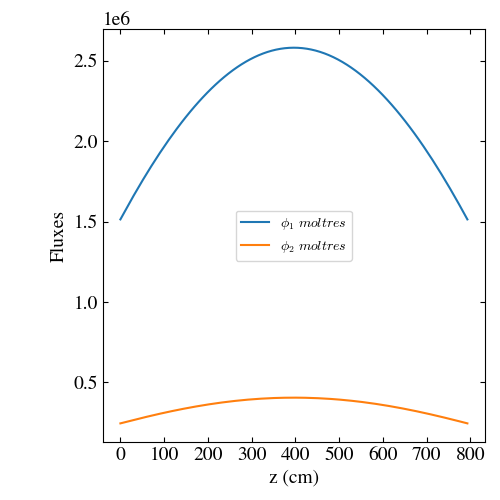
\includegraphics[width=\linewidth]{3D-unitcell2}
			\caption{Coolant centerline between points (0,0,0) and (0,0,793).}
		\end{subfigure}
		\hfill
		\caption{Group 1 and 2 axial fluxes in different locations of the unitcell at 10 msec.}
		\label{fig:3D-unitcell1}
	\end{figure}

\subsection{3D-unitcell-reflec}

	\begin{itemize}
		\item Input file: \textit{3D-unitcell-reflec.i}
		\item Mesh: \textit{3D-unitcell-reflec.msh}
		\item Transient problem.
	\end{itemize}

Figure \ref{fig:3D-unitcell-reflec} displays the geometry.
Figure \ref{fig:3D-unitcell-reflec1} shows the results.

	\begin{figure}[htbp!]
		\centering
		\begin{subfigure}[t]{0.4\textwidth}
			\centering
			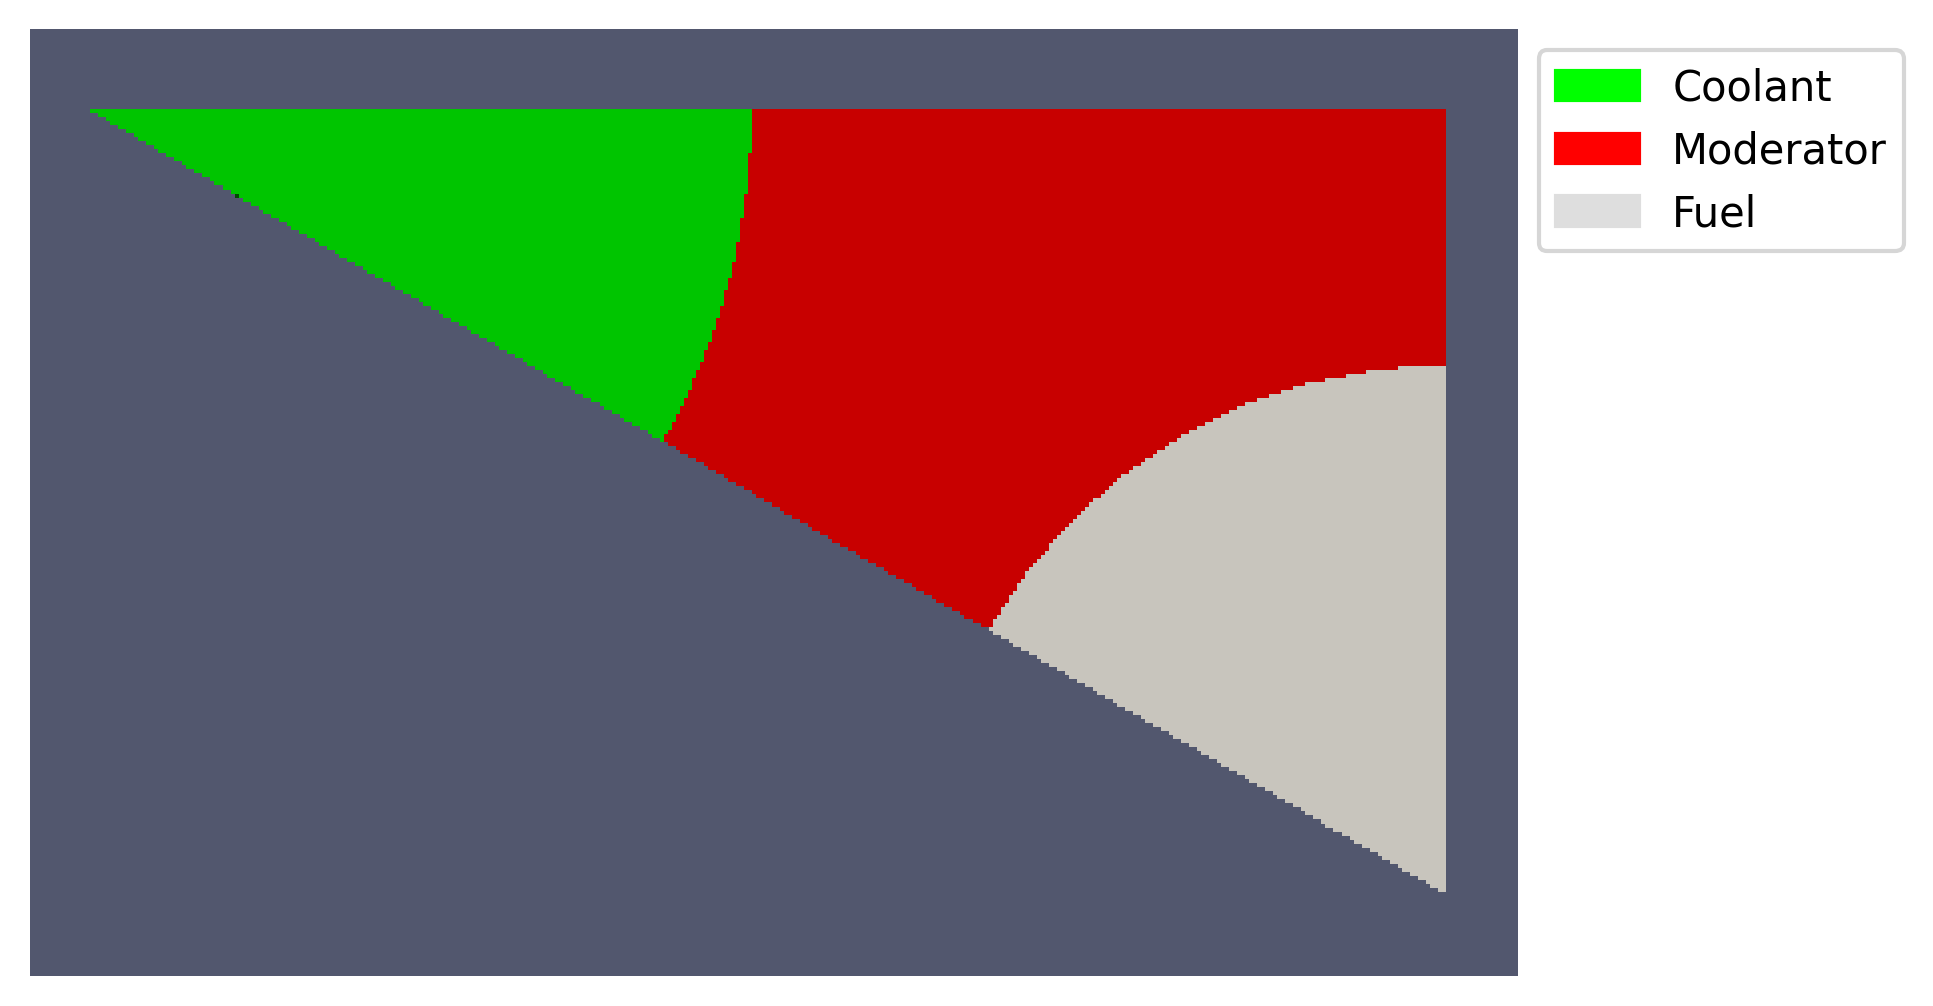
\includegraphics[width=\linewidth]{3D-unitcell-mesh1}
			\caption{XY-plane at z=400.}
		\end{subfigure}
		\begin{subfigure}[t]{0.4\textwidth}
			\centering
			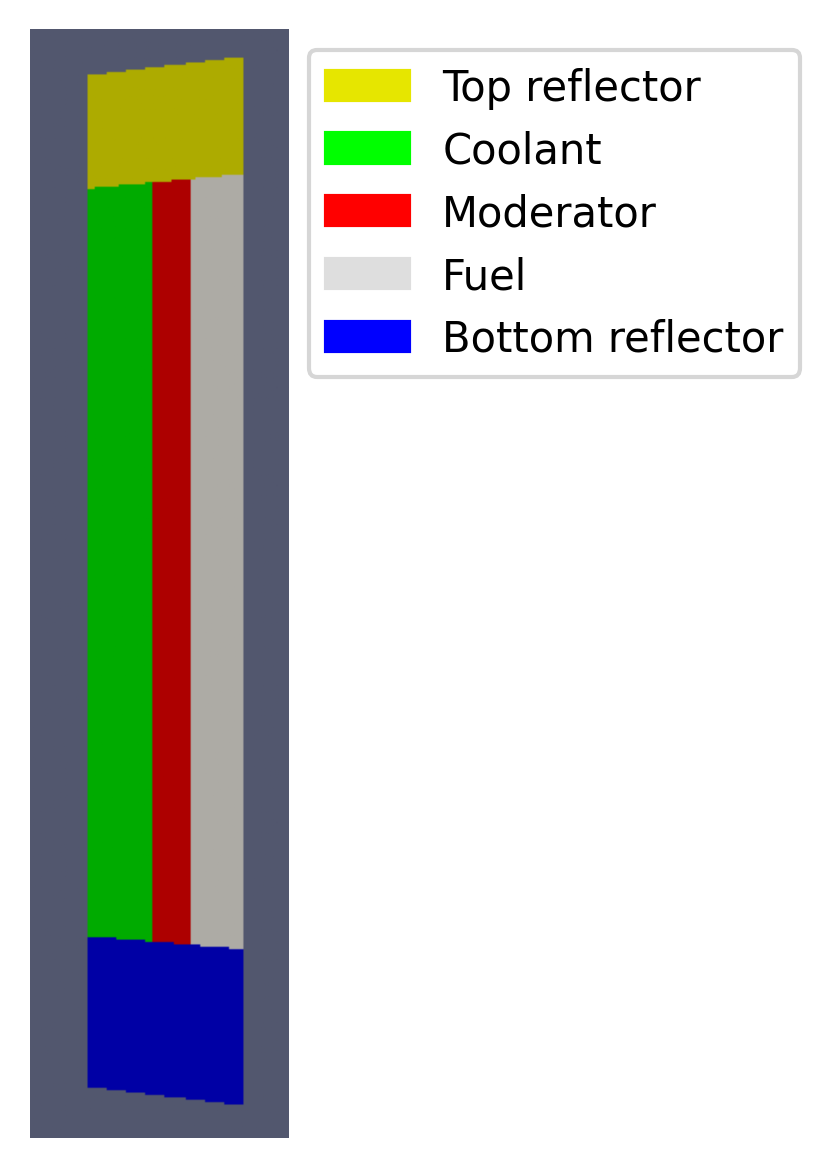
\includegraphics[width=\linewidth]{3D-unitcell-reflec-mesh}
			\caption{XZ-plane.}
		\end{subfigure}
		\hfill
		\caption{\textit{3D-unitcell-reflec} scaled down geometry.}
		\label{fig:3D-unitcell-reflec}
	\end{figure}

	\begin{figure}[htbp!]
		\centering
		\begin{subfigure}[t]{0.4\textwidth}
			\centering
			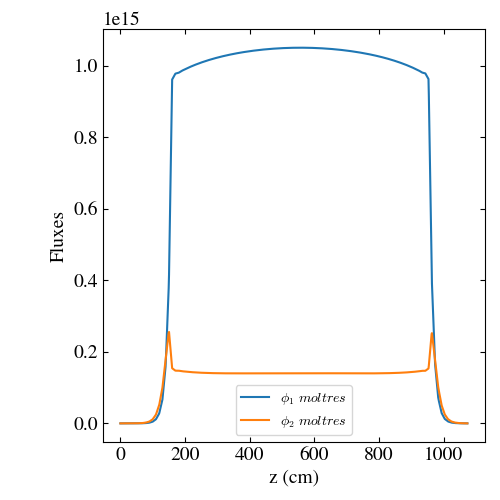
\includegraphics[width=\linewidth]{3D-unitcell-reflec1}
			\caption{Fuel centerline between points (1.628,-0.939,0) and (1.628,-0.939,1073).}
		\end{subfigure}
		\begin{subfigure}[t]{0.4\textwidth}
			\centering
			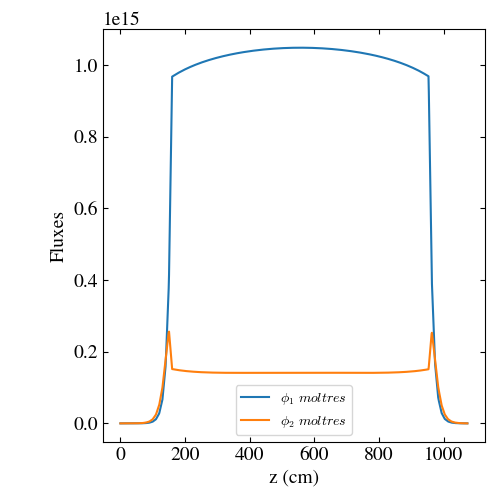
\includegraphics[width=\linewidth]{3D-unitcell-reflec2}
			\caption{Coolant centerline between points (1.628,-0.939,0) and (1.628,-0.939,1073).}
		\end{subfigure}
		\hfill
		\caption{Group 1 and 2 axial fluxes in different locations of the unitcell at 10 msec.}
		\label{fig:3D-unitcell-reflec1}
	\end{figure}

\subsection{3D-unitcell-reflec-homo}

	\begin{itemize}
		\item Input file: \textit{3D-unitcell-reflec-homo.i}
		\item Mesh: \textit{3D-unitcell-reflec.msh}
		\item Transient problem.
	\end{itemize}

Figure \ref{fig:3D-unitcell-reflec-homo} displays the geometry.
Figure \ref{fig:3D-unitcell-reflec-homo1} shows the results.

	\begin{figure}[htbp!]
		\centering
		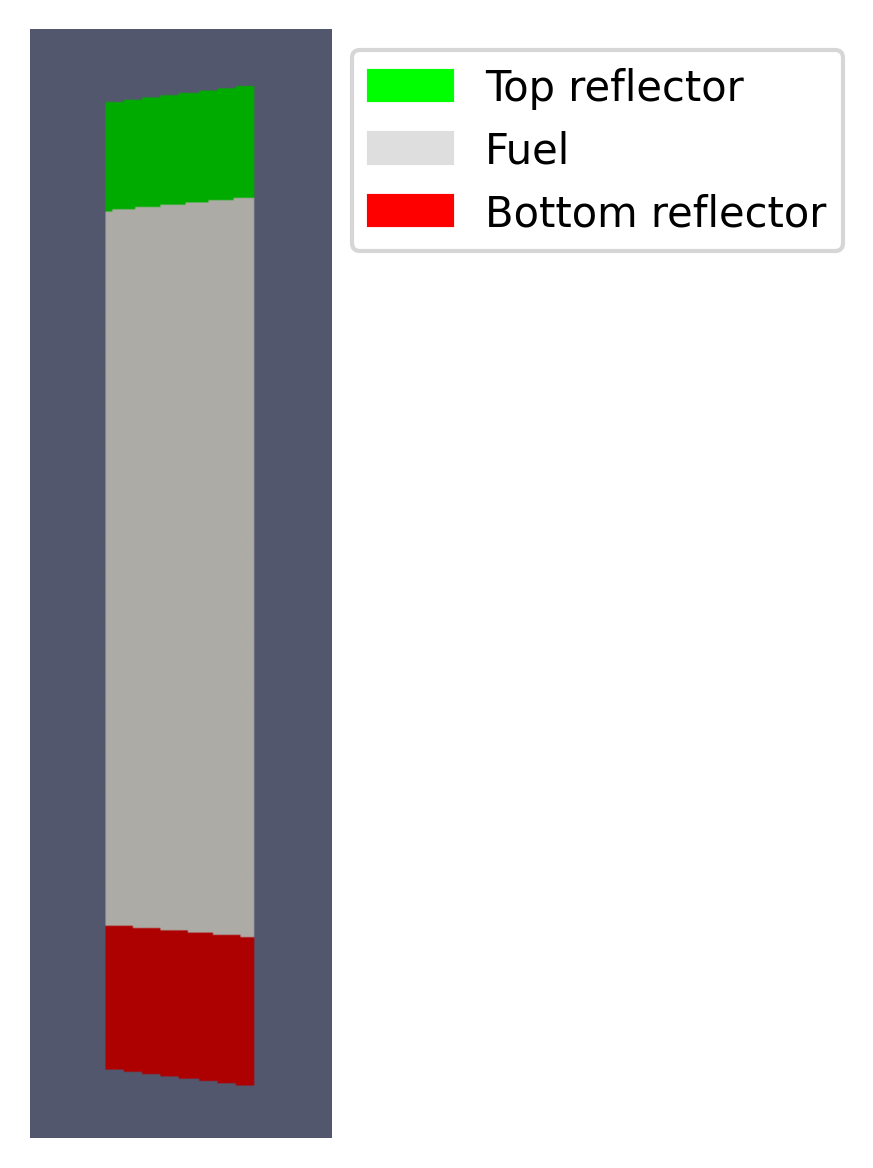
\includegraphics[height=5cm]{3D-unitcell-reflec-homo-mesh}
		\caption{\textit{3D-unitcell-reflec} scaled down geometry.}
		\label{fig:3D-unitcell-reflec-homo}
	\end{figure}

	\begin{figure}[htbp!]
		\centering
		
\includegraphics[height=8cm]{3D-unitcell-reflec-homo}
		\caption{Group 1 and 2 fluxes at 10 msec.}
		\label{fig:3D-unitcell-reflec-homo1}
	\end{figure}

\subsection{3D-assembly-homo-action}

	\begin{itemize}
		\item Input file: \textit{3D-assembly-homo-action.i}
		\item Mesh: \textit{3D-assembly-30deg-reflec.msh}
		\item Transient problem.
		\item Fuel, Moderator, and coolant are homogenized.
	\end{itemize}

Figure \ref{fig:3D-assembly-homo} displays the geometry.
Figure \ref{fig:3D-assembly-homo1} shows the results.

	\begin{figure}[htbp!]
		\centering
		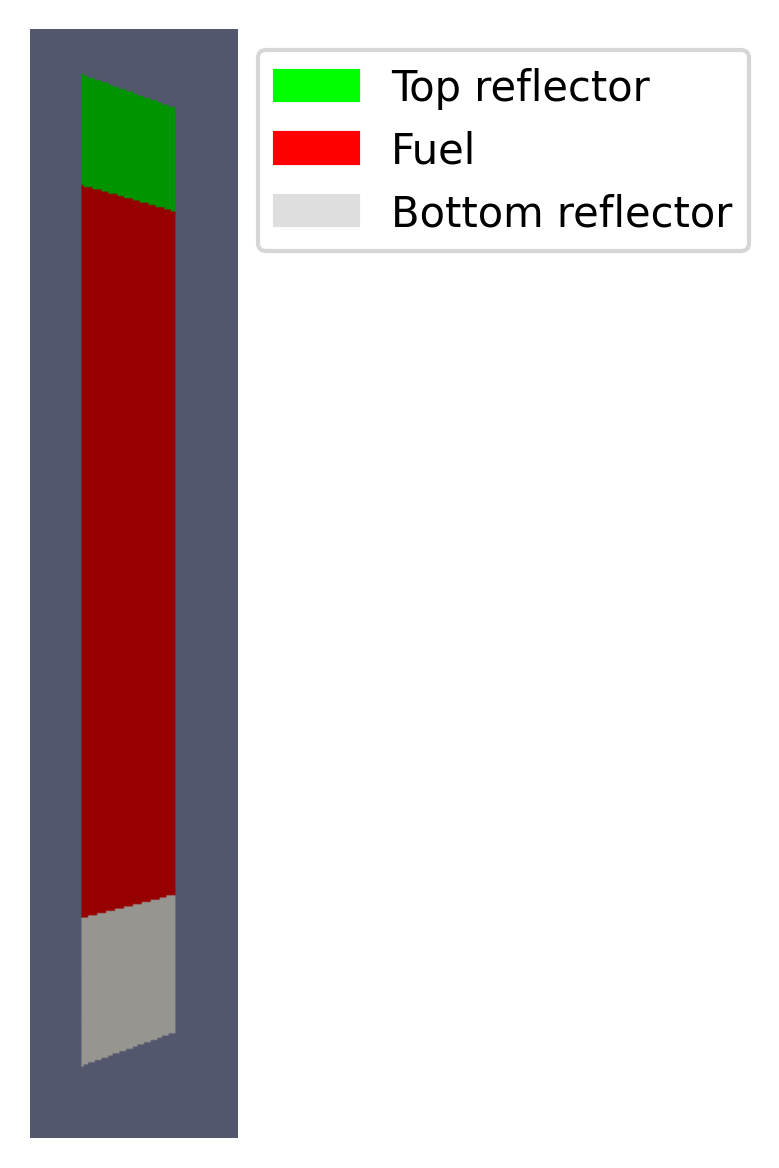
\includegraphics[height=5cm]{3D-assembly-homo-mesh}
		\caption{\textit{3D-assembly-30deg-reflec} scaled down geometry.}
		\label{fig:3D-assembly-homo}
	\end{figure}

	\begin{figure}[htbp!]
		\centering
		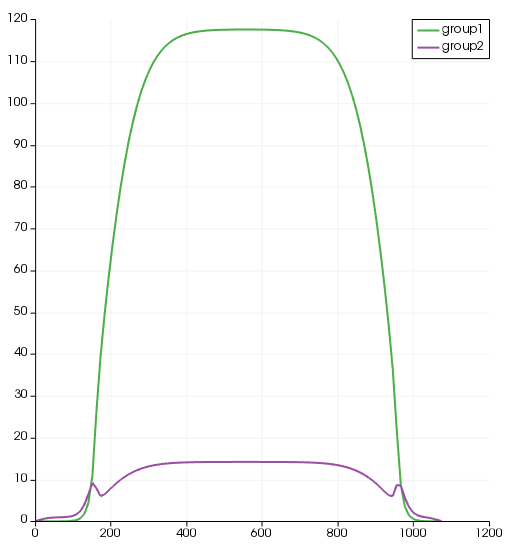
\includegraphics[height=8cm]{3D-assembly-homo}
		\caption{Group 1 and 2 axial flux at 1 msec.}
		\label{fig:3D-assembly-homo1}
	\end{figure}


\subsection{3D-fullcore-120-homo}

	\begin{itemize}
		\item Input file: \textit{3D-fullcore-120-homo.i}
		\item Mesh: \textit{3D-fullcore-120-homo.msh}
		\item Transient problem.
	\end{itemize}

Figure \ref{fig:3D-fullcore-homo} displays the geometry.
Figure \ref{fig:3D-fullcore-homo1} shows the results.

	\begin{figure}[htbp!]
		\centering
		\begin{subfigure}[t]{0.4\textwidth}
			\centering
		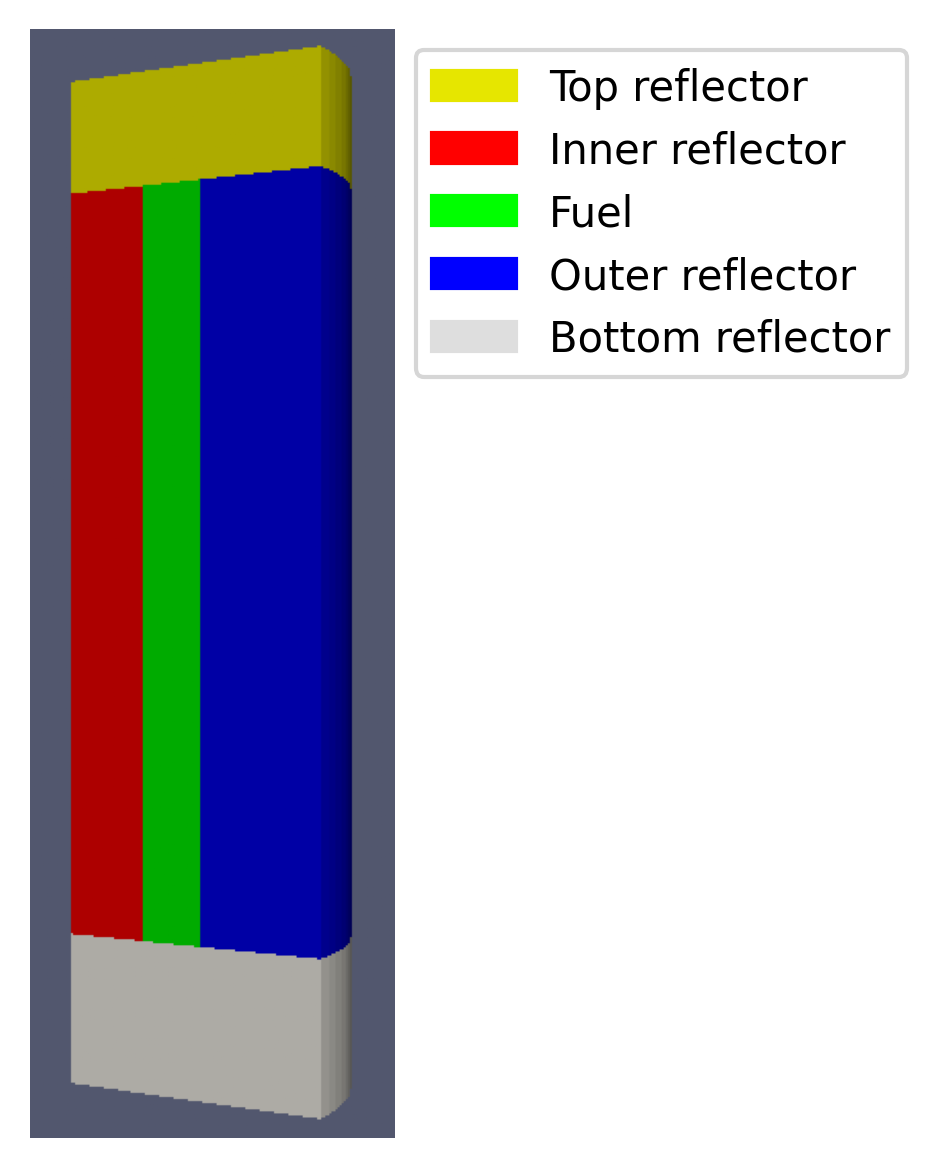
\includegraphics[height=5cm]{3D-fullcore-120-homo-mesh}
			\caption{XZ-plane.}
		\end{subfigure}
		\begin{subfigure}[t]{0.4\textwidth}
			\centering
		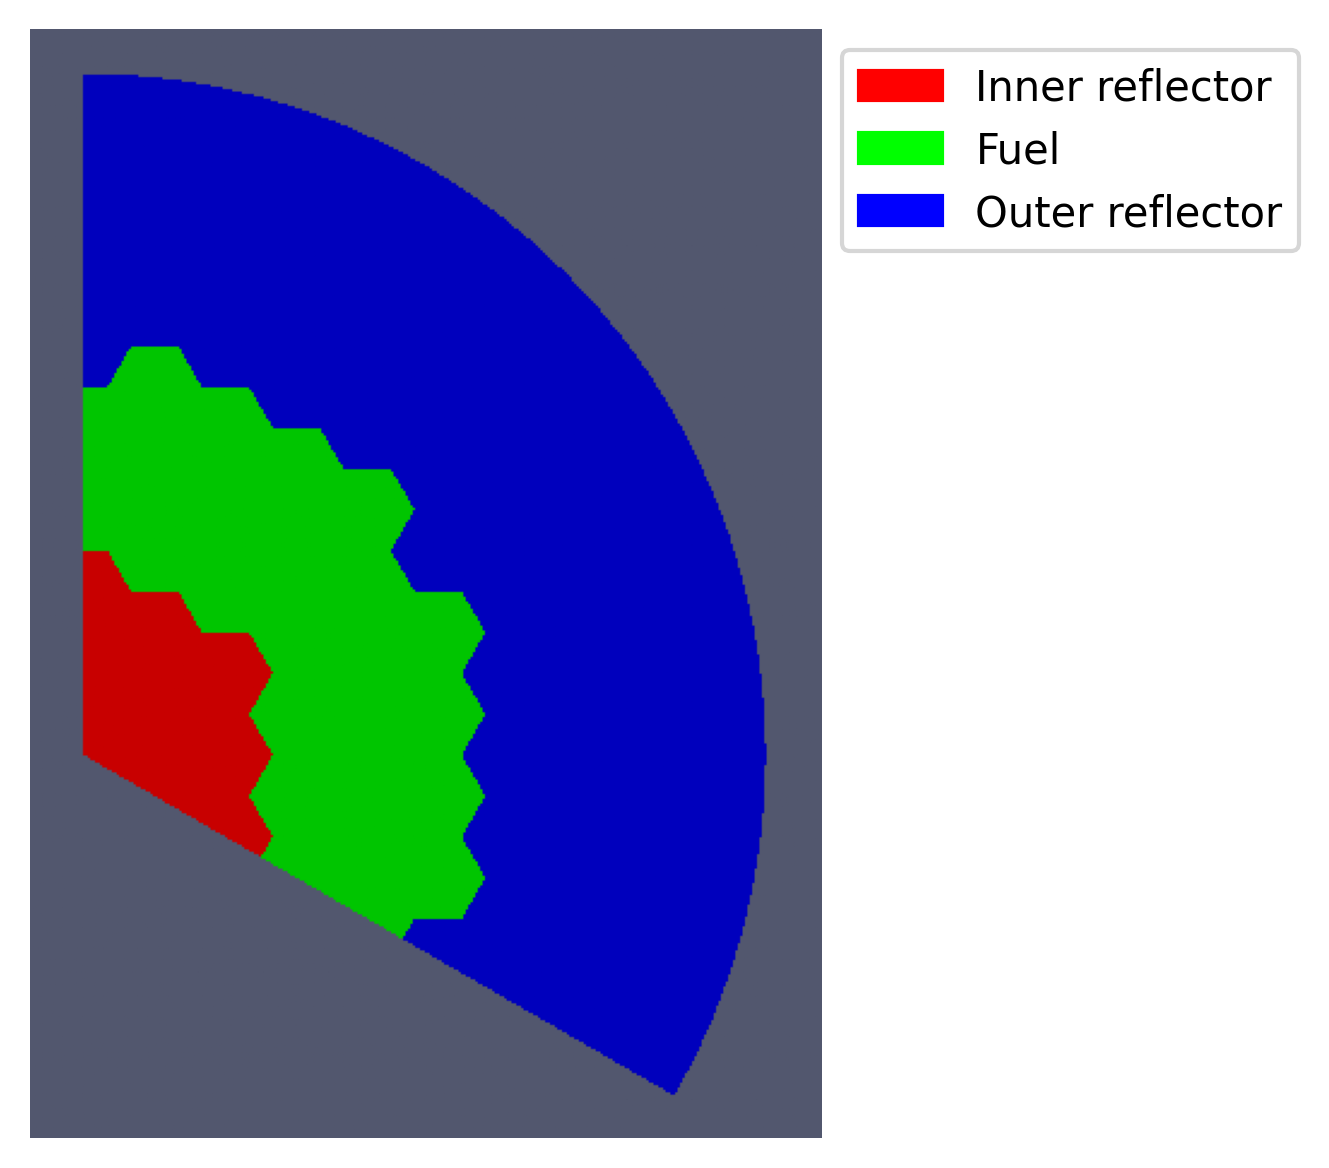
\includegraphics[height=5cm]{3D-fullcore-120-homo-mesh2}
			\caption{XY-plane.}
		\end{subfigure}
		\hfill
		\caption{\textit{3D-fullcore-120-homo} geometry.}
		\label{fig:3D-fullcore-homo}
	\end{figure}

	\begin{figure}[htbp!]
		\centering
		\begin{subfigure}[t]{0.4\textwidth}
			\centering
			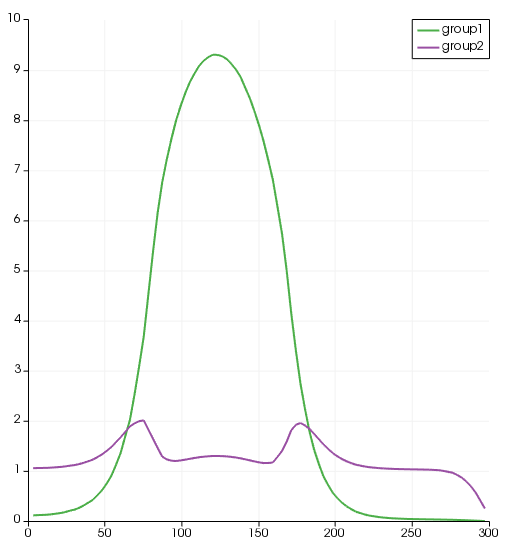
\includegraphics[width=\linewidth]{3D-fullcore-120-homoC1}
			\caption{Radial flux between points (0,0,400) and (300,0,400).}
		\end{subfigure}
		\begin{subfigure}[t]{0.4\textwidth}
			\centering
			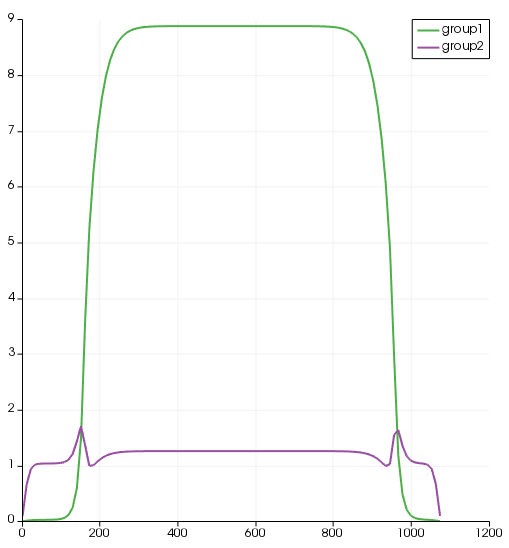
\includegraphics[width=\linewidth]{3D-fullcore-120-homoC2}
			\caption{Axial flux between points (120,-60,0) and (120,-60,1073).}
		\end{subfigure}
		\hfill
		\caption{Group 1 and 2 axial fluxes in different locations at 1 msec.}
		\label{fig:3D-fullcore-homo1}
	\end{figure}


\pagebreak
\bibliographystyle{plain}
% \bibliography{bibliography}

\end{document}
